\subsection{Kiểm định một mẫu cho hiệu năng Pixel\_Rate}

\subsubsection{Mục tiêu phân tích}
Nhóm thực hiện kiểm định này nhằm đánh giá xem năng lực xử lý điểm ảnh thực tế của các dòng GPU trong tập dữ liệu có đạt được ngưỡng công nghệ kỳ vọng là 40 GPixel/s hay không. Việc xác định này giúp nhóm có cái nhìn khách quan về vị thế hiệu năng của các sản phẩm so với tiêu chuẩn công nghiệp hiện hành.

\subsubsection{Thiết lập giả thuyết kiểm định}
Do dữ liệu đã được nhóm thực hiện biến đổi $\log(x + 1)$ ở bước tiền xử lý, giá trị mục tiêu 40 GPixel/s tương ứng với giá trị kiểm định trên thang đo log là: $\mu_0 = \ln(40 + 1) \approx 3.714$.
\begin{itemize}
    \item \textbf{Giả thuyết không ($H_0$):} $\mu = 3.714$.
    \item \textbf{Đối thuyết ($H_1$):} $\mu \neq 3.714$.
\end{itemize}

\subsubsection{Quy trình thực hiện và phân tích kịch bản}
Nhóm xây dựng quy trình lựa chọn phép thử dựa trên tính chất phân phối:
\begin{enumerate}
    \item \textbf{Kịch bản dữ liệu chuẩn:} Nếu kiểm định Shapiro-Wilk cho giá trị $p > 0.05$, nhóm sẽ sử dụng \textbf{One-sample T-test}.
    \item \textbf{Kịch bản dữ liệu không chuẩn:} Nếu $p \leq 0.05$, nhóm buộc phải sử dụng kiểm định phi tham số \textbf{Wilcoxon Signed-Rank Test} để bảo vệ kết quả khỏi sự ảnh hưởng của các giá trị ngoại lai và hình dạng phân phối lệch.
\end{enumerate}

\subsubsection{Triển khai các bước bằng code R và đánh giá kết quả}
\textbf{Bước 1: Kiểm tra tính chuẩn}
\begin{lstlisting}
shapiro.test(df_proc_log$Pixel_Rate)
\end{lstlisting}
\textbf{Kết quả:}
\begin{figure}[H]
    \centering
    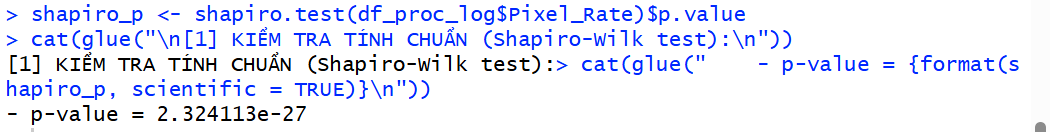
\includegraphics[width=1\linewidth]{../images/6.1.png}
    \caption{Kết quả kiểm định tính chuẩn cho Pixel\_Rate}
\end{figure}

\textbf{Đánh giá:} Kết quả trả về $p\text{-value} = 2.324 \times 10^{-27} < 0.05$. Do đó, nhóm bác bỏ giả định chuẩn và quyết định thực hiện bước tiếp theo bằng phương pháp Wilcoxon.

\textbf{Bước 2: Kiểm định chính và tính quy mô ảnh hưởng}
\begin{lstlisting}
res_one <- wilcox.test(df_proc_log$Pixel_Rate, mu = 3.714, conf.int = TRUE)
effectsize::cohens_d(df_proc_log$Pixel_Rate, mu = 3.714)
\end{lstlisting}

\textbf{Kết quả:}
\begin{figure}[H]
    \centering
    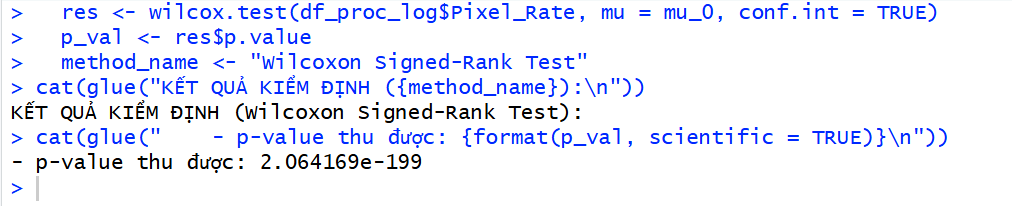
\includegraphics[width=1\linewidth]{../images/6.2.png}
    \caption{Kết quả thực thi kiểm định Wilcoxon Signed-Rank}
\end{figure}

\textbf{Đánh giá:} Với $p\text{-value} = 2.064 \times 10^{-199}$, nhóm có bằng chứng cực kỳ mạnh mẽ để bác bỏ $H_0$. Sự khác biệt giữa thực tế và mục tiêu không phải do ngẫu nhiên.

\subsubsection{Phân tích trực quan và kết luận ý nghĩa}
Nhóm đã vẽ biểu đồ mật độ nhằm xác nhận bằng mắt thường khoảng cách giữa trung bình mẫu thực tế và mục tiêu, đồng thời quan sát rõ hình dạng phân phối đa đỉnh của dữ liệu vốn là nguyên nhân dẫn đến việc vi phạm tính chuẩn ở bước trước.

\begin{figure}[H]
    \centering
    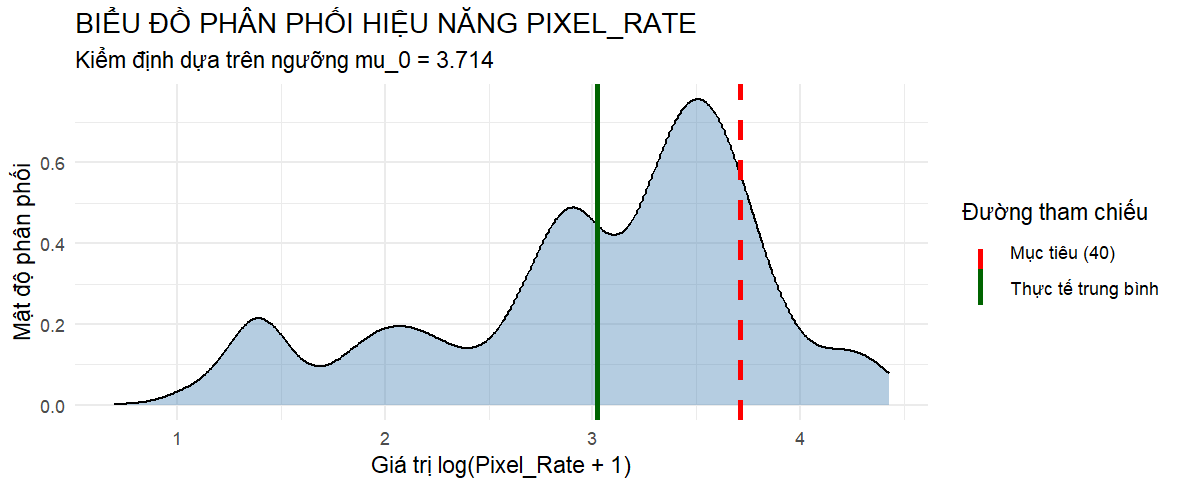
\includegraphics[width=1\linewidth]{../images/6.3.png}
    \caption{Biểu đồ mật độ Pixel\_Rate thực tế so với đường mục tiêu (Đỏ)}
    \label{fig:density_1sample}
\end{figure}

\textbf{Phân tích chi tiết biểu đồ và kết luận:}
\begin{itemize}
    \item \textbf{Về hình ảnh:} Đường kẻ dọc màu xanh (Trung bình thực tế) nằm lệch hẳn sang bên trái đường đứt đoạn màu đỏ (Mục tiêu 3.714). Phân phối xuất hiện nhiều đỉnh tập trung quanh dải 2.5 - 3.5, cho thấy hiệu năng phần lớn GPU trong tập dữ liệu đều thấp hơn kỳ vọng.
    \item \textbf{Ý nghĩa thực tế:} Kết hợp với chỉ số \textbf{Cohen's d = 0.881} (mức ảnh hưởng \textbf{Lớn}), nhóm kết luận rằng hiệu năng GPU thực tế đang tụt hậu một khoảng cách công nghệ đáng kể so với ngưỡng 40 GPixel/s lý tưởng.
\end{itemize}